\documentclass[11pt,a4paper]{article}
\usepackage[utf8]{inputenc}
\usepackage{babel}
\usepackage{graphicx}
\usepackage{geometry}
\usepackage{float}
\usepackage{hyperref}
\usepackage{booktabs}
\geometry{top=2.5cm, bottom=2.5cm, left=3cm, right=3cm}

\title{\textbf{Procesamiento de Imágenes de Plantas para la Detección de Plagas}\\
\Large Primer Parcial: Descripción y Preprocesamiento}
\author{Ingeniería en Computación\\
Dra. Verónica Rodríguez López}
\date{\today}

\begin{document}

\maketitle

\begin{abstract}
Este reporte detalla el análisis y las técnicas de preprocesamiento aplicadas al \textit{New Plant Diseases Dataset}. Se aborda la identificación de las características de las imágenes, los problemas inherentes a su captura y el diseño de un pipeline de filtros de Procesamiento Digital de Imágenes (PDI) modularizado. Este enfoque emplea principios de diseño S.O.L.I.D. y algoritmos avanzados para aislar el tejido vegetal y mejorar el contraste clínico de las lesiones fúngicas y patológicas.
\end{abstract}

\section{Datos: Descripción del Conjunto de Imágenes}
El \textit{New Plant Diseases Dataset} fue obtenido del repositorio de Kaggle. Está diseñado para entrenar modelos computacionales en el diagnóstico de enfermedades agrícolas. A continuación, se resumen los elementos identificados en el análisis del conjunto:

\begin{table}[H]
    \centering
    \renewcommand{\arraystretch}{1.2}
    \begin{tabular}{@{}ll@{}}
        \toprule
        \textbf{Característica} & \textbf{Valor Observado} \\ \midrule
        Formato de las imágenes & \texttt{.jpg} (JPEG) \\
        Resolución espacial & $256 \times 256$ píxeles \\
        Profundidad de color & 24 bits (3 canales RGB, 8 bits/canal) \\
        Número total de imágenes & 87,900 imágenes \\
        Partición (Split) & Entrenamiento: 70,295 $\vert$ Validación: 17,572 $\vert$ Prueba: 33 \\
        Categorías (Clases) & 38 clases diagnosticadas + 1 clase \texttt{test\_unlabeled} \\ \bottomrule
    \end{tabular}
    \caption{Resumen estadístico y técnico del dataset analizado.}
    \label{tab:dataset_stats}
\end{table}

\begin{figure}[H]
    \centering
    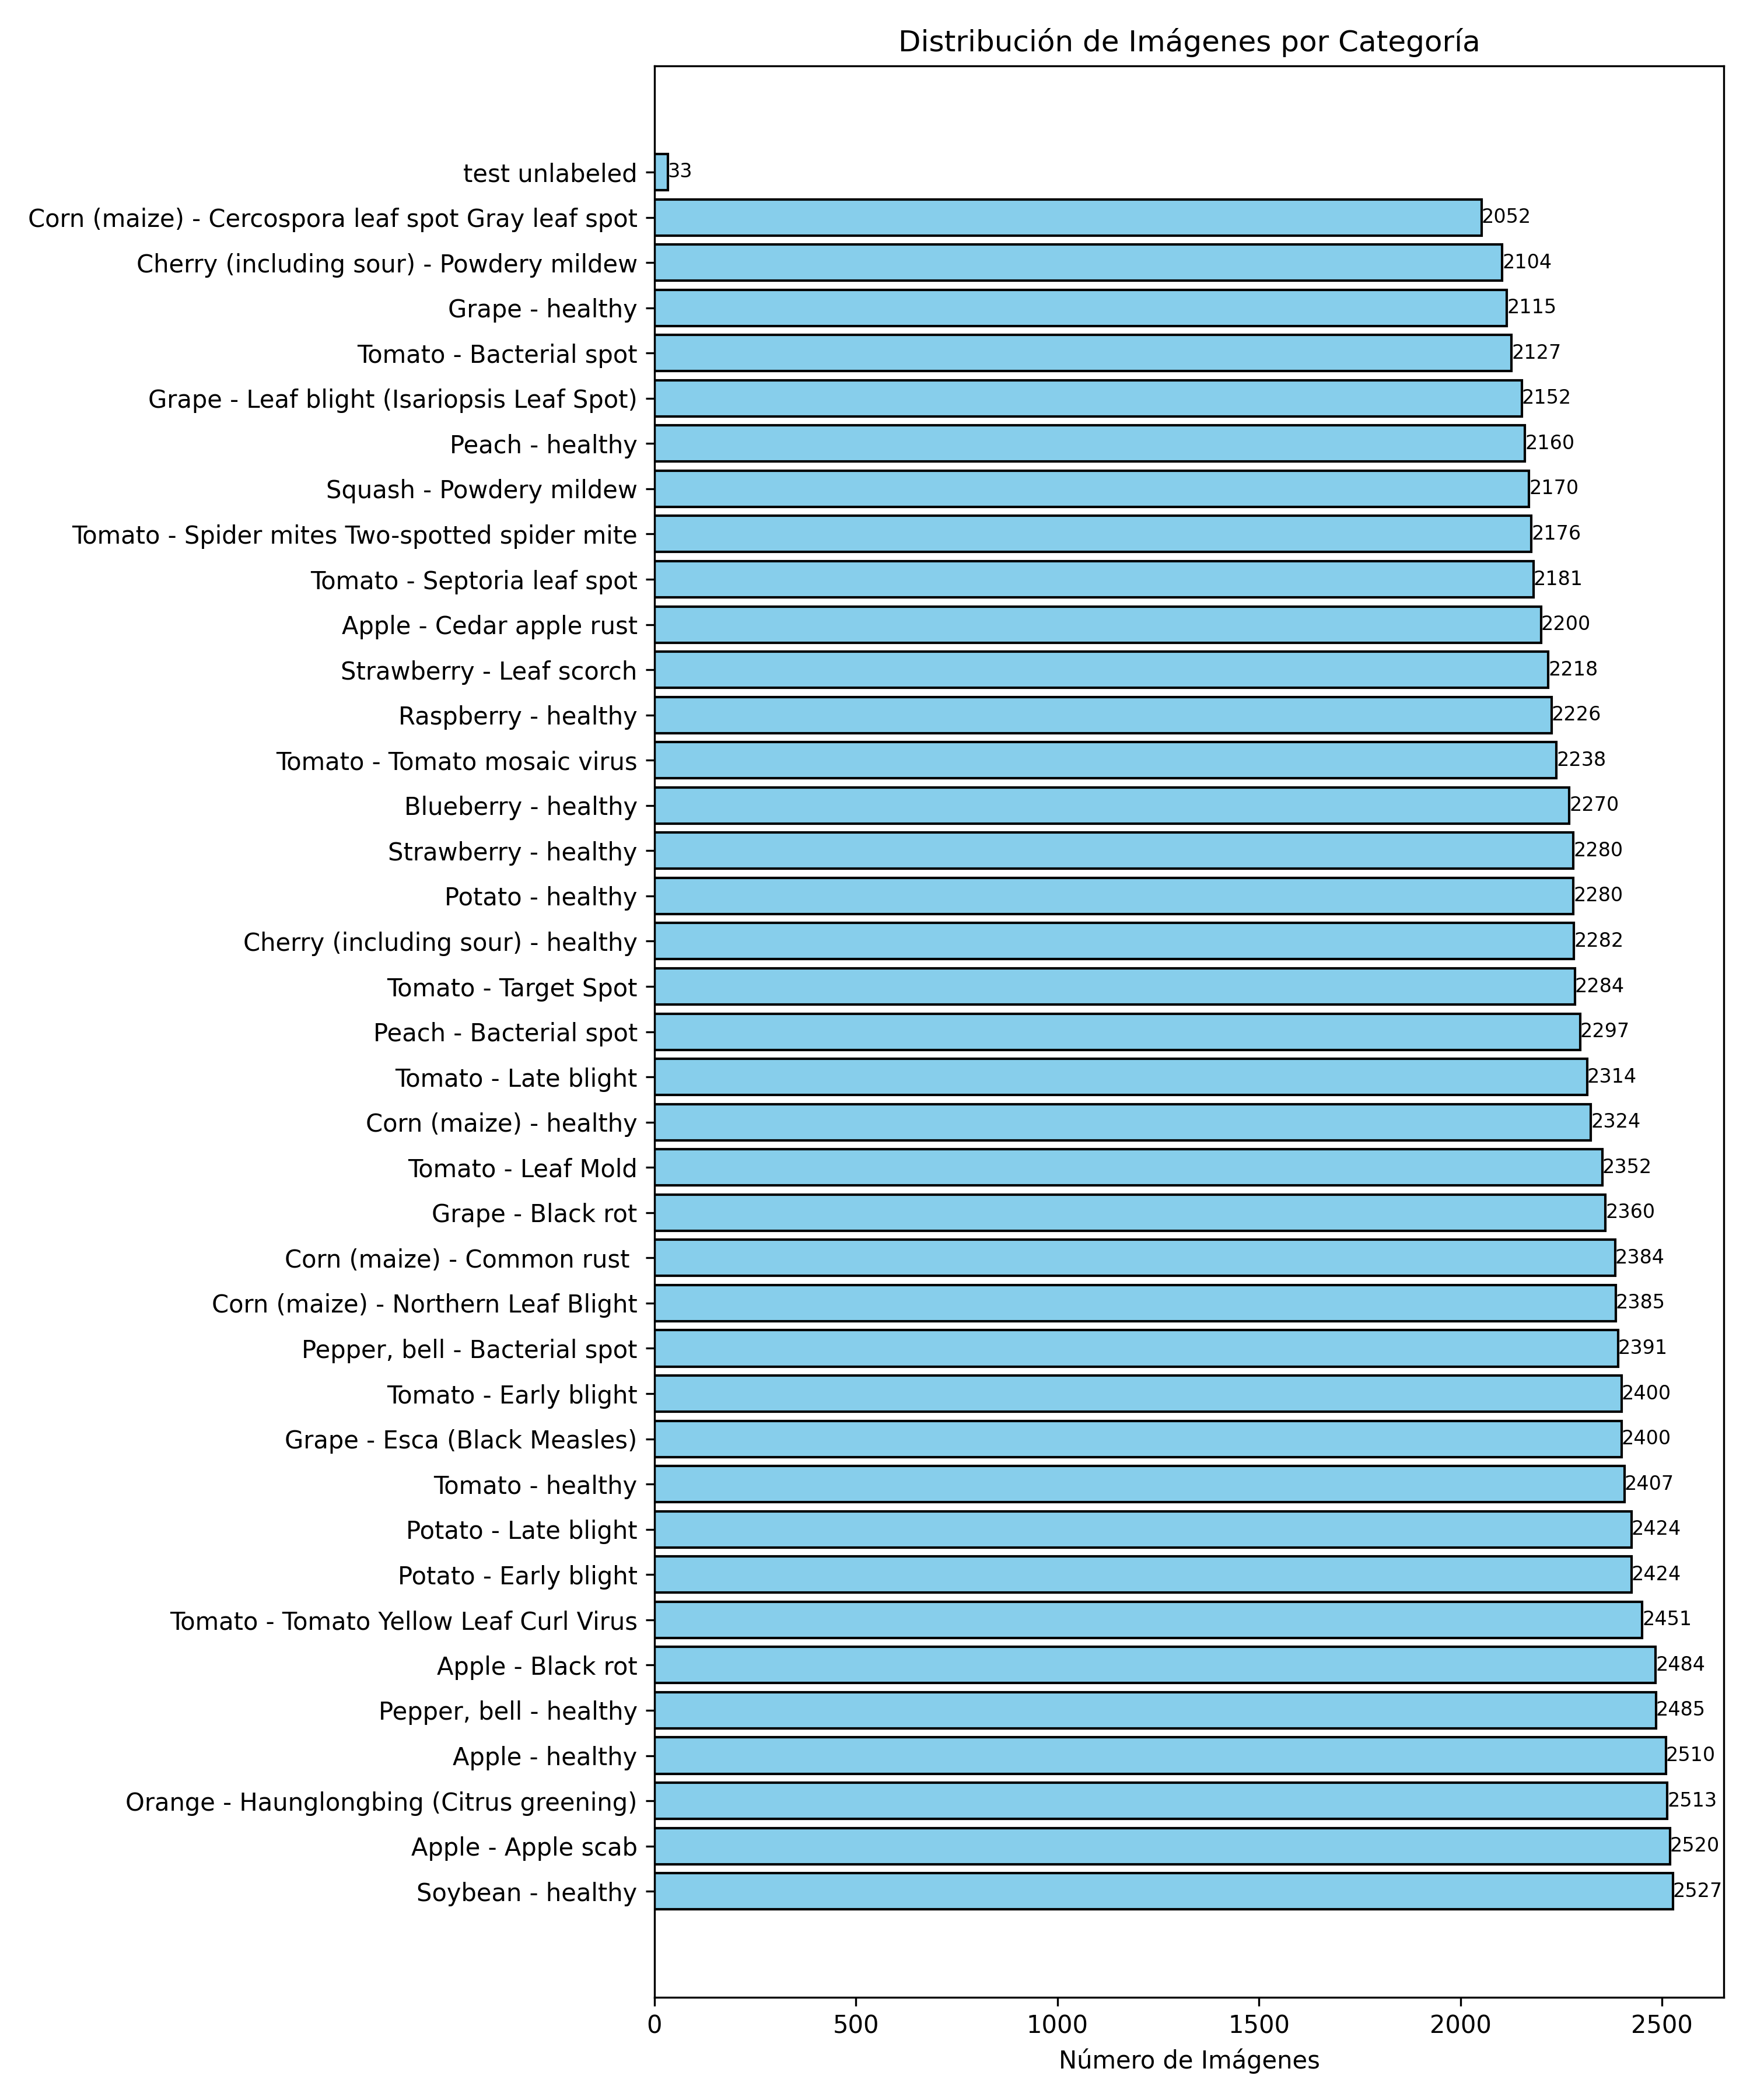
\includegraphics[width=0.95\textwidth]{resultados/distribucion_clases.png}
    \caption{Distribución del número de imágenes por categoría en el dataset. Como se observa, la distribución de clases se encuentra balanceada rondando las 2,000 y 2,500 imágenes por categoría.}
    \label{fig:distribucion_clases}
\end{figure}

\section{Preprocesamiento: Problemas y Metodología}

\subsection{Problemas Encontrados}
Al inspeccionar las imágenes, se identificaron los siguientes retos fotométricos y espaciales:
\begin{itemize}
    \item \textbf{Interferencia de Fondo y Variación de Tamaños:} Muchas hojas fueron fotografiadas sobre cartulinas de laboratorio con texturas y arrugas. Además, en la captura original cruda existe \textbf{variación en el tamaño} de las imágenes, lo cual se resolvió estandarizando todo el conjunto a $256 \times 256$ píxeles.
    \item \textbf{Intensidades, Color y Escala de Grises:} Se presentan variaciones en el número de intensidades por problemas de subexposición y sombras. Además, aunque el conjunto está en RGB, algunas imágenes presentan bajo nivel de croma asemejándose a \textbf{imágenes en escala de grises}, lo que requiere separar la luminancia de la crominancia (espacio CIELAB).
    \item \textbf{Ruido Espacial:} Se detectó \textbf{ruido} de sensor y artefactos de compresión en las transiciones de alta frecuencia (bordes de la hoja).
\end{itemize}

\subsection{Metodología y Diagrama de Flujo (Pipeline S.O.L.I.D.)}

La arquitectura del sistema fue refactorizada utilizando el patrón \textit{Composite} para encadenar operaciones sin acoplar dependencias. El diagrama a continuación describe el flujo gráfico de la información:

\begin{figure}[H]
    \centering
    \fbox{
    \begin{minipage}{0.8\textwidth}
    \centering
    \textbf{1. Imagen Original} (RGB, $256\times256$) \\[1em]
    $\downarrow$ \\[1em]
    \textbf{2. Filtro Bilateral} (Suavizado $\sigma_c, \sigma_s$) \quad \textbf{+} \quad \textbf{2b. Máscara ExG} (Segmentación Otsu) \\[1em]
    $\downarrow$ (sobre rama principal) \\[1em]
    \textbf{3. Ecualización CLAHE} (Canal $L^*$ en Lab) \\[1em]
    $\downarrow$ \\[1em]
    \textbf{4. Unsharp Masking} (Realce de bordes) \\[1em]
    $\downarrow$ \\[1em]
    \textbf{5. Fusión Final} (Tejido Realzado con Máscara ExG)
    \end{minipage}
    }
    \caption{Diagrama de flujo del pipeline de preprocesamiento propuesto (S.O.L.I.D.).}
    \label{fig:flowchart}
\end{figure}

Las técnicas aplicadas paso a paso son:
\begin{enumerate}
    \item \textbf{Filtrado Bilateral:} Suaviza el ruido conservando estrictamente los contornos de las lesiones en lugar de difuminarlos.
    \item \textbf{Ecualización Adaptativa (CLAHE):} Amplifica el contraste dinámico localmente, mejorando la visibilidad del patrón de la enfermedad sin saturación global.
    \item \textbf{Realce Unsharp:} Utiliza sustracción gaussiana ponderada para acentuar las nervaduras y micelios patológicos.
    \item \textbf{Segmentación ExG:} Usa la fórmula geométrica de Exceso de Verde ($2G - R - B$) junto con umbralización automática de Otsu para suprimir completamente la interferencia del fondo.
\end{enumerate}

\section{Resultados y Comparación Visual}

Al ejecutar el módulo de visualización, generamos una matriz comparativa aplicando aisladamente cada método frente a nuestro pipeline segmentado recomendado. 

\begin{figure}[H]
    \centering
    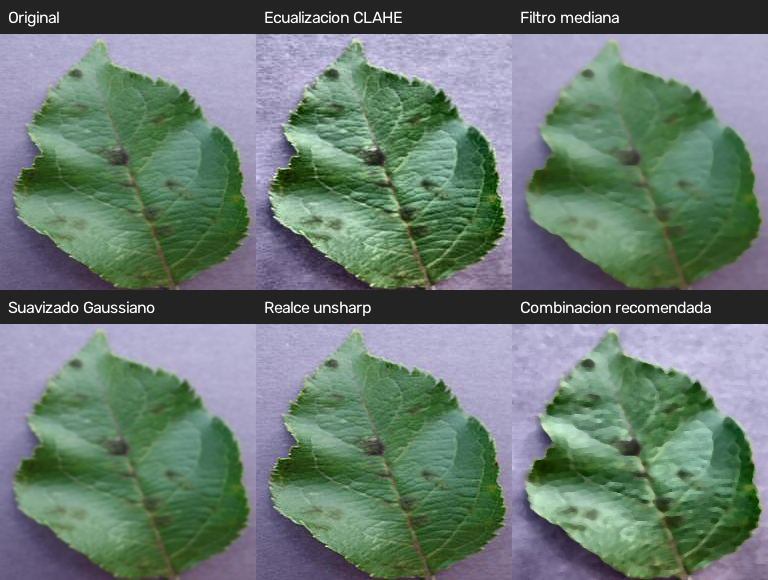
\includegraphics[width=0.65\textwidth]{resultados/filtros_01.png}
    
    \vspace{0.5em}
    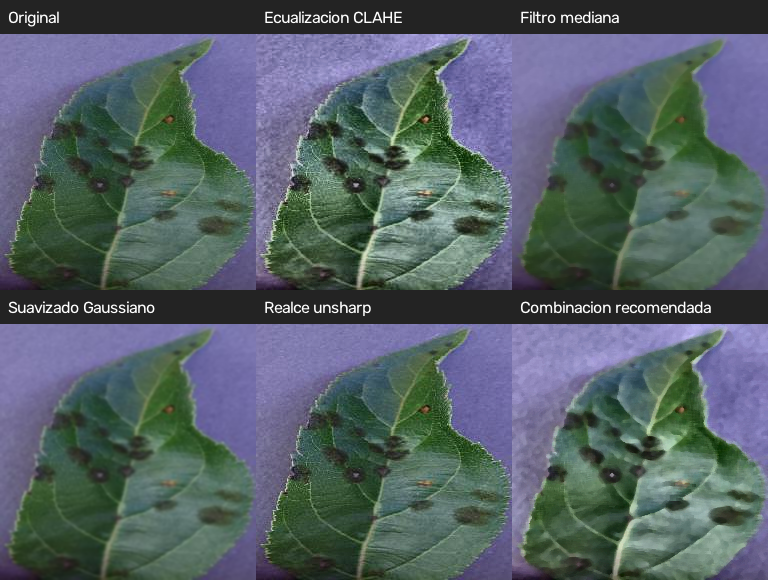
\includegraphics[width=0.65\textwidth]{resultados/filtros_02.png}
    
    \vspace{0.5em}
    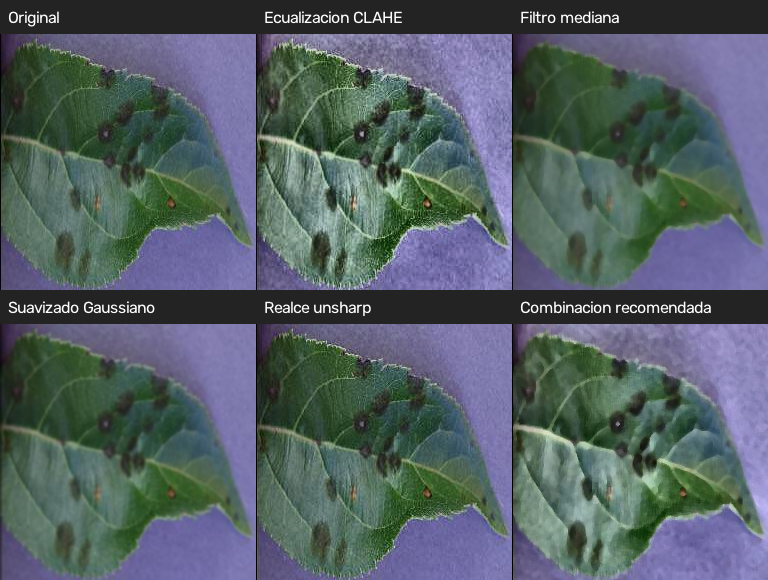
\includegraphics[width=0.65\textwidth]{resultados/filtros_03.png}
    
    \caption{Resultados obtenidos al aplicar diversos filtros. Se muestran 3 imágenes comparativas que evidencian cómo filtros básicos como Mediana degradan la textura foliar, mientras que el Pipeline S.O.L.I.D. propuesto focaliza el realce aislando la hoja.}
    \label{fig:comparacion1}
\end{figure}

\textbf{Justificación Clínica y Técnica:}
La \textit{Combinación Recomendada} con soporte S.O.L.I.D. resultó ser superior porque evita artefactos de posterización destructivos. Al aislar la hoja con el índice \textit{ExG}, evitamos que las ecualizaciones subsiguientes conviertan el fondo inerte en ruido predominante, focalizando el aprendizaje automático exclusivamente en las patologías foliares.

\section{Referencias}
\begin{thebibliography}{9}
\bibitem{gonzalez}
Gonzalez, R. C., \& Woods, R. E. (2018). \textit{Digital Image Processing} (4th ed.). Pearson.
\bibitem{kaggle}
New Plant Diseases Dataset. Kaggle. Disponible en: \url{https://www.kaggle.com/datasets/vipoooool/new-plant-diseases-dataset}
\end{thebibliography}

\end{document}
